\documentclass{article}

\usepackage{xcolor}
\usepackage{amsmath}
\usepackage{amssymb}
\usepackage{graphicx}
\usepackage{algorithm2e}


\newcommand{\rami}[1]{\textbf{\color{red}[[RAMI: #1]]}}
\newcommand{\thyag}[1]{\textbf{\color{blue}[[THYAG: #1]]}}


\title{LLMNET: a library for extracting functional [brain] networks from large language models}

\author{Thyag Raj and Rami Puzis}




\begin{document}

\maketitle


\begin{abstract}
\rami{write last}   
\end{abstract}

\section{Introduction}
\rami{write last}   




\section{Background}
\subsection{Functional brain networks}
\rami{Write here things you learn about fMRI and brain networks.}

Many functional brain networks are created from resting state fMRI scans~\cite{van2010exploring}. 
\rami{Make sure that every special term is explained before it is used. 
For example, before making the above claim, fMRI must be explained.}

\subsection{Large language models}
\rami{Write here things you learn about LLMs.}


\section{Algorithms}
\rami{Description of your own work including pseudocode goes here.}


\section{API reference}


\section{Benchmarks}
\rami{Here, you describe the main results when there will be results.}

Figure~\ref{fig:my_label} presents something as a function of something. 
\rami{Always include axis names in charts!!!}


\begin{figure}
    \centering
    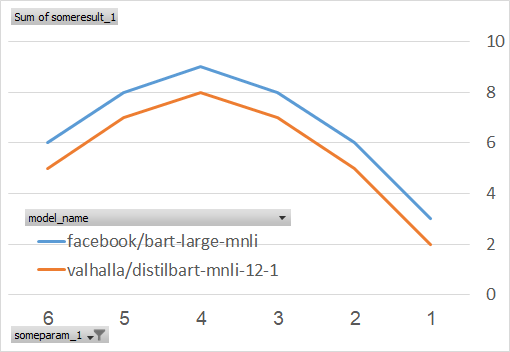
\includegraphics[width=0.5\columnwidth]{results/example_chart.png}
    \caption{Example figure with some fictional results}
    \label{fig:my_label}
\end{figure}


\bibliographystyle{unsrt}
\bibliography{bib}


\end{document}